\chapter{O mundo que faltou}\label{cap:faltou}

A travessia fechou com um preço em cada pergunta. O andar que começa aqui vira a conta para o outro
lado e pergunta o que **não** se compra, começando pela mais dura: de que serve uma proteção
calibrada no que já se viu, quando o prejuízo é decidido pelo mundo que não se viu?

\section{O pior dia como teto}

A resposta natural, e a que quase todo mundo dá, é dimensionar a proteção pelo pior dia do registro.
Ela tem duas falhas, e as duas se medem.

A primeira é que o pior dia do registro não é um teto, e a chance de perdê-lo é exata. Com um ano de
histórico e um ano pela frente, a probabilidade de que apareça um dia pior do que tudo o que já se
viu é de \numRecordeProbabilidade{} --- meio. A chance de que seja já o dia seguinte é de
\numRecordeDoProximo{}, medida sobre o registro de \numRecordeIndiceDias{} dias do índice.

A segunda é o tamanho do salto quando o recorde cai. No índice, medido em \numRecordeIndiceDias{} dias, o pior dia perde \numRecordeIndicePior{} contra
\numRecordeIndiceSegundo{} do segundo pior, numa razão de \numRecordeIndiceRazao{}; no Ibovespa, em
\numRecordeIbovespaDias{} dias, o pior perde \numRecordeIbovespaPior{} contra
\numRecordeIbovespaSegundo{} do segundo, numa razão de \numRecordeIbovespaRazao{}; e no Bitcoin, em
\numRecordeBitcoinDias{} dias, o pior dia perde \numRecordeBitcoinPior{} contra
\numRecordeBitcoinSegundo{} do segundo, uma razão de \numRecordeBitcoinRazao{}. Um recorde novo não
chega encostado no antigo.

\section{A conta exata}

As duas probabilidades acima saem de uma contagem, e a contagem é a mesma do primeiro capítulo.

\begin{proposicao}[o recorde e o que vem depois]\label{prop:recorde}
Se \emph{n} dias observados e \emph{m} dias por vir forem permutáveis, então a probabilidade de que
o próximo dia supere o recorde dos \emph{n} já vistos é $1/(n+1)$, e a de que algum dos \emph{m}
dias por vir o supere é $m/(n+m)$. O número esperado de recordes em \emph{n} dias é o harmônico
$H(n)$, que cresce como o logaritmo de \emph{n}.
\end{proposicao}

\begin{proof}
Sob permutabilidade, os $n+m$ valores são permutáveis, de modo que o maior deles está em qualquer
das $n+m$ posições com a mesma chance. Dizer que algum dos $m$ últimos é o maior é dizer que o
máximo caiu no futuro, o que tem probabilidade $m/(n+m)$; com $m=1$ sai $1/(n+1)$. Para a contagem
de recordes, o dia $k$ é recorde exatamente quando o maior dos $k$ primeiros está na posição $k$,
o que tem probabilidade $1/k$; somando sobre $k$ chega-se ao harmônico.
\end{proof}

A proposição dá o preço de uma coisa que ninguém vende: a chance de o mundo que faltou ser pior do
que o mundo que se viu. Com mil dias de histórico ela é de \numRecordeEsperadoMil{} recordes ao
longo do caminho, e com \numRecordeDiasPorMundo{} dias ela é de \numRecordeEsperadoMundo{} --- o
logaritmo cresce devagar, e é por isso que a memória compra tão pouco.

\section{A conta conferida, e o dado real}

A conta foi conferida por sorteio, em \numRecordeSorteios{} sorteios e em \numRecordeSementes{}
mundos: com sessenta e sessenta dias de cada lado, a fração em que o futuro bateu o passado foi de
\numRecordeMedidoSessenta{}; com um ano de cada lado, \numRecordeMedidoAno{}; contra os
\numRecordeProbabilidade{} previstos nos dois casos. Num mundo simulado que não muda, os recordes
medidos foram de \numRecordeParado{}, com dispersão de \numRecordeParadoDispersao{}, contra os
\numRecordeEsperadoMundo{} da conta.

No dado real os recordes são menos do que a conta diz: \numRecordeIndiceConta{} no índice,
\numRecordeIbovespaConta{} no Ibovespa e \numRecordeBitcoinConta{} no Bitcoin, contra
\numRecordeIndiceEsperado{}, \numRecordeIbovespaEsperado{} e \numRecordeBitcoinEsperado{}. A
diferença tem explicação declarada: os dias ruins do mercado chegam em cachos, e quando o recorde
cai, ele costuma cair junto com outros dias no mesmo cacho --- o que reduz a contagem sem reduzir a
perda. A permutabilidade supõe dias independentes, e os dias deste livro não são.

\begin{figure}[htbp]
  \centering
  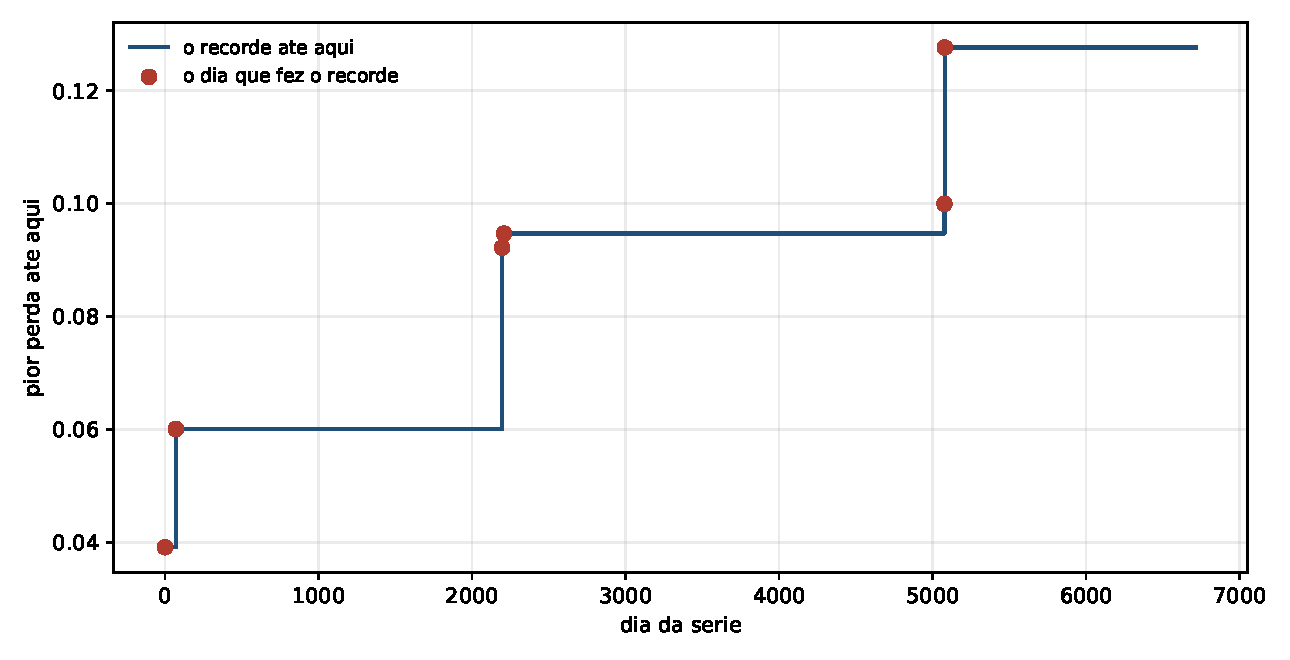
\includegraphics[width=\linewidth]{figuras/E15_mundo_que_faltou_1.pdf}
  \caption{A escada do recorde no índice: a pior perda até cada dia, e os dias que ergueram o
    recorde. São poucos degraus, e cada um deles é um mundo que ainda não tinha sido visto.}
  \label{fig:escada}
\end{figure}

\section{O que a mudança faz com a conta}

Falta o controle que separa a falha do dado da falha do mundo. A conta supõe permutabilidade, e
permutabilidade é a hipótese de que o mundo não muda. Num mundo que muda, ela deixa de valer, e o
lado para o qual ela erra é conhecido.

\begin{table}[htbp]
  \centering
  \small
  \begin{tabular}{lrrr}
    \hline
    mudança no & recordes & dias por cima & razão dos \\
    meio da série & medidos & do recorde & extremos \\
    \hline
    nenhuma & \numRecordeRecordesSemMudanca & \numRecordeFracaoSemMudanca & \numRecordeRazaoSemMudanca \\
    vinte por cento & \numRecordeRecordesVintePorCento & \numRecordeFracaoVintePorCento & \numRecordeRazaoVintePorCento \\
    metade & \numRecordeRecordesMetade & \numRecordeFracaoMetade & \numRecordeRazaoMetade \\
    o dobro & \numRecordeRecordesDobro & \numRecordeFracaoDobro & \numRecordeRazaoDobro \\
    o triplo & \numRecordeRecordesTriplo & \numRecordeFracaoTriplo & \numRecordeRazaoTriplo \\
    \hline
  \end{tabular}
  \caption{A conta dos recordes é sempre a mesma, \numRecordeEsperadoMundo{}, porque ela não sabe da
    mudança. A última coluna é a razão entre o extremo de depois da mudança e o de antes, e confere
    com o fator posto no mundo.}
  \label{tab:mudanca}
\end{table}

Num mundo parado, a fração de dias que passam por cima do recorde anterior é
\numRecordeFracaoSemMudanca{}, que é ruído. Num mundo que dobra no meio da série, ela é de
\numRecordeFracaoDobro{}, e num que triplica, \numRecordeFracaoTriplo{}. Os recordes medidos sobem de
\numRecordeRecordesSemMudanca{} para \numRecordeRecordesDobro{} e \numRecordeRecordesTriplo{}, sempre
contra os \numRecordeEsperadoMundo{} da conta.

\begin{figure}[htbp]
  \centering
  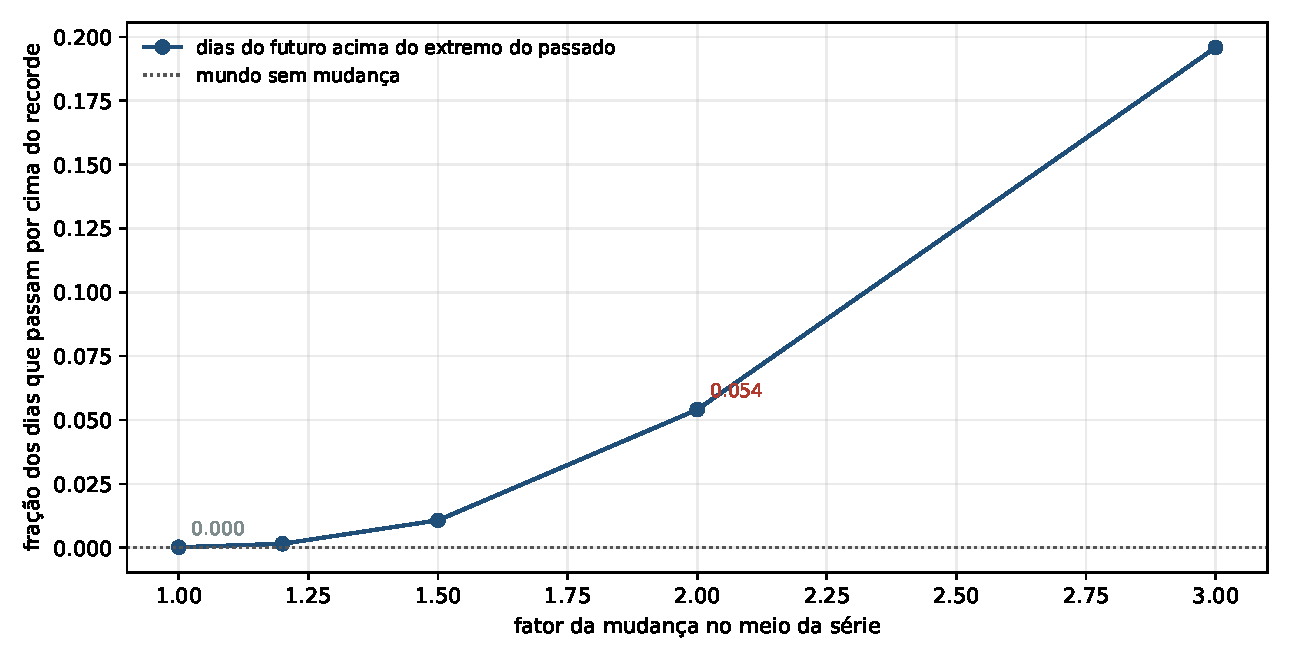
\includegraphics[width=\linewidth]{figuras/E15_mundo_que_faltou_2.pdf}
  \caption{A fração dos dias seguintes que passam por cima do recorde de tudo o que veio antes,
    contra o tamanho da mudança. A linha pontilhada é o mundo que não muda.}
  \label{fig:alem}
\end{figure}

\section{O que fica}

Fica a resposta do primeiro pedaço do andar. O mundo que faltou fica fora do registro, e nenhuma
janela, nenhum dado e nenhum dinheiro o trazem para dentro. A conta exata diz apenas **quanto** ele
pode custar --- a probabilidade $m/(n+m)$ de que o futuro passe por cima de tudo o que se viu. Isso já
vale a pena saber, porque transforma um susto em um preço declarado.

E fica o limite da conta, medido: ela vale enquanto o mundo não muda. Quando muda, a fração de dias
que passam por cima do registro sai do ruído e vai a \numRecordeFracaoDobro{} e a
\numRecordeFracaoTriplo{}, e a conta de permutabilidade --- que é a mesma do primeiro capítulo ---
erra para o lado otimista. Quem dimensiona pelo pior dia do registro, e acrescenta a margem que a
conta sugere, está protegido contra o mundo que não mudou e descoberto contra o que mudou.

O próximo pedaço do andar é o espelho deste. Aqui se mediu o que o registro não tem porque ainda não
aconteceu; a pergunta seguinte é o que o registro não tem porque foi **apagado** --- e se há algum
preço que traga de volta o que a memória do sistema já jogou fora.
